%-----------------------------------------------------------------------
%
%   UFRJ  - Universidade Federal do Rio de Janeiro
%   COPPE - Coordena��o dos Programas de P�s-gradua��o em Engenharia
%   PEE   - Programa de Engenharia El�trica
%
%   COE-835  Controle adaptativo
%
%   Relat�rio da simula��o
%                                                         Ramon R. Costa
%                                                         05/out/09, Rio
%-----------------------------------------------------------------------
\documentclass[11pt,a4paper]{article}
\usepackage[latin1]{inputenc} %pacote para utilizar palavras acentuadas
\usepackage{amsmath,amssymb}  %pacotes do AMS
\usepackage{latexsym}         %pacote para incluir s�mbolos (ex.\Box)
\usepackage{fancybox,fancyhdr}%pacote com frescuras
\usepackage{graphicx}         %pacote para incluir figuras tipo eps
\usepackage[portuguese]{babel}
\usepackage{xcolor}
\usepackage{float}
\usepackage[a4paper]{hyperref}% Make sure it comes last of your loaded packages
\hypersetup{
  verbose,
  plainpages=false,
  bookmarks=true,
  colorlinks=true,
  linkcolor=blue
}

%----------------------------------------------------------------------
%
%   Macros utilizados no LATEX
%                                                       Ramon R. Costa
%                                                       13/out/17, Rio
%----------------------------------------------------------------------
\newcount\m
\newcount\n

\def\twodigits#1{\ifnum #1<10 0\fi \number#1}

\def\hours{\n=\time \divide\n 60
    \m=-\n \multiply\m 60 \advance\m \time
    \twodigits\n:\twodigits\m}

\def\hora{\hours}

\def\fim{
  \medskip
  \begin{center}
    \rule[1mm]{30mm}{0.14mm}$\diamond$\rule[1mm]{30mm}{0.14mm}
  \end{center}
}

%----------------------------------------------------------------------
% A4 paper size & margins
\setlength {\textheight}    {25cm}%
\setlength {\textwidth}     {17.5cm}%
\setlength {\parindent}     {0mm}%
\setlength {\parskip}       {1mm}%
\setlength {\topmargin}     {-14mm}%
\setlength {\oddsidemargin} {-6mm}%
\setlength {\evensidemargin}{-6mm}%
\setlength {\columnsep}     {6mm}%

%----------------------------------------------------------------------
\def\codigo{COE-835}
\def\disciplina{Controle adaptativo}
\def\periodo{3o. período/2017}
\def\professor{Ramon}

\newcommand{\BOX}[1]{
  \framebox{{\color{magenta}\rule[-3mm]{1mm}{9mm}} ~~$\displaystyle
  \begin{aligned} #1 \end{aligned}$~~}\pagestyle{plain}
}

\newcommand{\RED}[1]{\colorbox{white}{\textcolor{red}{#1}}}
%\newcommand{\WoR}[1]{\colorbox{red}{\textcolor{white}{#1}}}
\newcommand{\BLU}[1]{\colorbox{white}{\textcolor{blue}{#1}}}
\newcommand{\GRE}[1]{\colorbox{green}{\textcolor{black}{#1}}}
\newcommand{\HI}[1]{\colorbox{yellow}{\textcolor{black}{#1}}}  %% Highlithed text

\newcommand{\estrela}[1]{
  \def\TXT{\RED{$\bigstar$ }}
  \hspace*{5mm}\TXT \hfill
  \parbox[t]{ \textwidth - \widthof{\TXT} - 5mm}{#1}
  \par
}

\def\Ltwo{\mbox{${\mathcal L}_2$}}
\def\Linf{\mbox{${\mathcal L}_\infty$}}

\newcommand{\sign}{\mbox{sign}}

\newcommand{\equacao}[2]{
  \makebox[40mm][l]{#1 \dotfill}: \quad \parbox[t]{8cm}
	{\begin{equation} \displaystyle
  \begin{aligned}
    #2
  \end{aligned} \end{equation}} \\
}

\newcommand{\sref}[1]{Section~\ref{#1}}
\newcommand{\fref}[1]{Fig.~\ref{#1}}
\newcommand{\tref}[1]{Table~\ref{#1}}
\newcommand{\thref}[1]{Theorem~\ref{#1}}
\newcommand{\aref}[1]{Assumption~\ref{#1}}
\newcommand{\norm}[1]{\left\lVert#1\right\rVert}
%\renewcommand{\qedsymbol}{}
\newcommand{\rev}[1]{{\color{red}#1}}
%\newcommand{\mat}[1]{\begin{bmatrix}#1\end{bmatrix}}

\newtheorem{remark}{Remark}
\newtheorem{lemma}{Lema}
\theoremstyle{plain}
\newtheorem{theorem}{Teorema}
%----------------------------------------------------------------------


\begin{document}
%---------------------------------------------------------------------
\pagestyle{fancy}%
\renewcommand{\headrulewidth}  {0.4pt}%
\renewcommand{\footrulewidth}  {0.4pt}%
\lhead{\bfseries{Relat�rio do Trabalho 1}}%
\chead{}%
\rhead{\bfseries\thepage}%
\lfoot{}%
\cfoot{}%
\rfoot{[\hours] \quad \today}%
%---------------------------------------------------------------------
\begin{center}
  \huge{COE-835  Controle  adaptativo}  \\[20mm]

  \Large{Simula��es do Trabalho 1} \\[20mm]
\end{center}

Algoritmo: \quad \HI{Gradiente normalizado}

\bigskip%
Caso: \quad \parbox[t]{10cm}{
  $~n = 1$ \quad (ordem da planta) \\[2mm]
  $n^* = 1$ \quad (grau relativo) \\[2mm]
  $n_p = 1$ \quad (\# de par�metros) \\[20mm]
}

%---------------------------------------------------------------------
\tableofcontents
\newpage
%---------------------------------------------------------------------
%---------------------------------------------------------------------
\section{Resumo das equa��es do m�todo}

Abaixo, resumimos algumas das principais equa��es utilizadas no m�todo.

\vspace{20mm}

\noindent

\equacao{Planta}
  {\dot{y} = a_p y + u \label{eq:planta}}

\equacao{Modelo}
  {\dot{y}_m = -a_m y_m + r \label{eq:ref_model}}

\equacao{Erro de sa�da}
  {e_0 = y - y_m \label{eq:error}}

\equacao{Lei de controle}
  {u(t) = k(t) \, y + r \label{eq:ctrl_law}}

\equacao{Filtro}
  { F(s) = \frac{1}{s+a_f} \label{eq:filter}}

%\equacao{Ganho ideal (matching gain)}
  %{k^* = -a_p-a_m \label{eq:ideal_gain}}

\equacao{Ganho estimado}
  {k(t) = -\hat{a}_p-a_m \label{eq:est_gain}}

\equacao{Sa�da filtrada}
	{\phi = F(s) \odot y }

\equacao{Par�metro estimado}
	{\theta = a_f + \hat{a}_p \quad ou \quad
	\theta = \hat{a}_p}

\equacao{Predi��o da sa�da}
	{\hat{y} = \theta \, \phi + F(s) \odot u
	\label{eq:pred_saida} }

\equacao{Erro de predi��o}
	{\epsilon = \hat{y} - y \label{eq:pred_error}}

\equacao{Lei de adapta��o}
  {\dot{\theta} = - \frac{\gamma \epsilon \phi}{m^2} \,, \quad m^2 = 1+\phi^2 \label{eq:adpt_law}}

 \newpage
%---------------------------------------------------------------------
\section{Prova da limita��o de $\dot{\varepsilon}/m$}

Utilizando as equa��es do sistema, a din�mica do erro � expressa por:
%
\begin{flalign}
\dot{e}_0 &= \dot{y}_p - \dot{y}_m \nonumber \\
&= -a_m \, e_0 + \tilde{\theta} \, y_p \,,
\end{flalign}
%
ou ainda:
%
\begin{flalign}
e_0 &= \mathcal{L}^{-1}\left\{\frac{1}{s+a_m}\right\} \circledast ( \tilde{\theta}\,y_p ) \nonumber \\ 
&= \mathcal{L}^{-1}\left\{\frac{1}{s+a_m}\right\} \circledast (\theta\,y_p) - \theta^* \, \zeta \,,
\end{flalign}
%
onde $\tilde{\theta} = \theta - \theta^*$, $\theta^*$ � o ganho de realimenta��o ideal, o operador $\mathcal{L}^{-1}\{*\}$ denota a transformada de Laplace inversa e $\circledast$ denota a opera��o de \textit{convolu��o}.
%
Assim, o erro de estimativa pode ser escrito como:
%
\begin{flalign}
\varepsilon &= e_0 - \hat{e} \nonumber \\ 
&=\mathcal{L}^{-1}\left\{\frac{1}{s+a_m}\right\} \circledast (\theta \, y_p) - \theta^* \, \zeta - \mathcal{L}^{-1}\left\{\frac{1}{s+a_m}\right\} \circledast (\theta \, y_p) + \theta \, \zeta \nonumber \nonumber \\
&= \tilde{\theta} \, \zeta \,.
\label{eq:erro_est}
\end{flalign}

A seguinte candidata � fun��o de Lyapunov � proposta:
%
\begin{equation}
2V(\tilde{\theta}) = \gamma^{-1} \, \tilde{\theta}^2 \ge 0
\end{equation}

Derivando e utilizando a lei de adapta��o proposta, tem-se:
%
\begin{flalign}
\dot{V} &= \gamma^{-1} \, \tilde{\theta} \, \dot{\theta} \nonumber \\
&= - \frac{\varepsilon^2}{m^2} \leq 0 \,,
\end{flalign}
%
onde \eqref{eq:erro_est} foi utilizado. Como $\dot{V}$ � apenas negativa \textit{semi-definida}, mostra-se que $\tilde{\theta} \in \mathcal{L}_{\infty}$.

\begin{lemma}
Sejam $a,b \in \mathbb{R}$ e $m^2 = 1+a^2+b^2$. Ent�o:
%
\begin{flalign}
\norm{\frac{a}{m}} \leq 1 \,, \quad \forall a,b \in \mathbb{R} \,, \nonumber \\
\norm{\frac{b}{m}} \leq 1 \,, \quad \forall a,b \in \mathbb{R} \,. \nonumber
\end{flalign}
%
\end{lemma}

Dividindo \eqref{eq:erro_est} por $m = \sqrt{1+\zeta^2+\dot{\zeta}^2}$, obtemos:
%
\begin{flalign}
\frac{\varepsilon}{m} = \tilde{\theta} \, \frac{\zeta}{m} \,.
\label{eq:erro_est2}
\end{flalign}

De acordo com o Lema 1 (para $a = \zeta$, $b=\dot{\zeta}$), $\norm{\zeta/m} \leq 1$ e, como $\tilde{\theta} \in \mathcal{L}_{\infty}$, ent�o 
$\varepsilon/m \in \mathcal{L}_{\infty}$.
%
A lei de controle pode ser expressa por:
\begin{equation}
\dot{\theta} = \dot{\tilde{\theta}} = - \gamma \, \underbrace{\frac{\varepsilon}{m}}_{\in \mathcal{L}_{\infty}} \, \frac{\zeta}{m} \,.
\end{equation}

Como $\varepsilon/m \in \mathcal{L}_{\infty}$ e pelo Lema 1 $\norm{\zeta/m} \leq 1$, ent�o $\dot{\tilde{\theta}} \in \mathcal{L}_{\infty}$.
%
Finalmente, derivando \eqref{eq:erro_est} no tempo e divindo por $m$, obtemos:
%
\begin{flalign}
\frac{\dot{\varepsilon}}{m} = \underbrace{\dot{\tilde{\theta}}}_{\in \mathcal{L}_{\infty}} \, \frac{\zeta}{m} + \underbrace{\tilde{\theta}}_{\in \mathcal{L}_{\infty}} \, \frac{\dot{\zeta}}{m} \,.
\label{eq:erro_est3}
\end{flalign}

Novamente utilizando o Lema 1, mostra-se que os sinais constituintes de $\dot{\varepsilon}/m$ s�o limitados, e portanto $\dot{\varepsilon}/m \in \mathcal{L}_{\infty}$. $\blacksquare$
 \newpage
%---------------------------------------------------------------------
\section{Diagramas de blocos}


\begin{figure}[H]
  \centering
  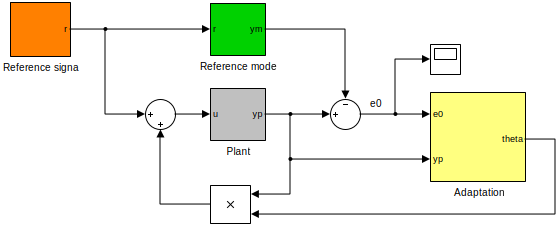
\includegraphics[width=14cm]{figs/blocks/MRAC_111_8_5.pdf}
  \caption{Diagrama de blocos do sistema. \quad
  (Model: \HI{\texttt{MRAC-111.mdl}}) }
\end{figure}

%---------------------------------------------------------------------
\bigskip%
\begin{figure}[H]
  \centering
  \includegraphics[scale=0.8]{figs/blocks/plant.pdf}
  \caption{Diagrama de blocos da planta.}
\end{figure}

%---------------------------------------------------------------------
\bigskip%
\begin{figure}[H]
  \centering
  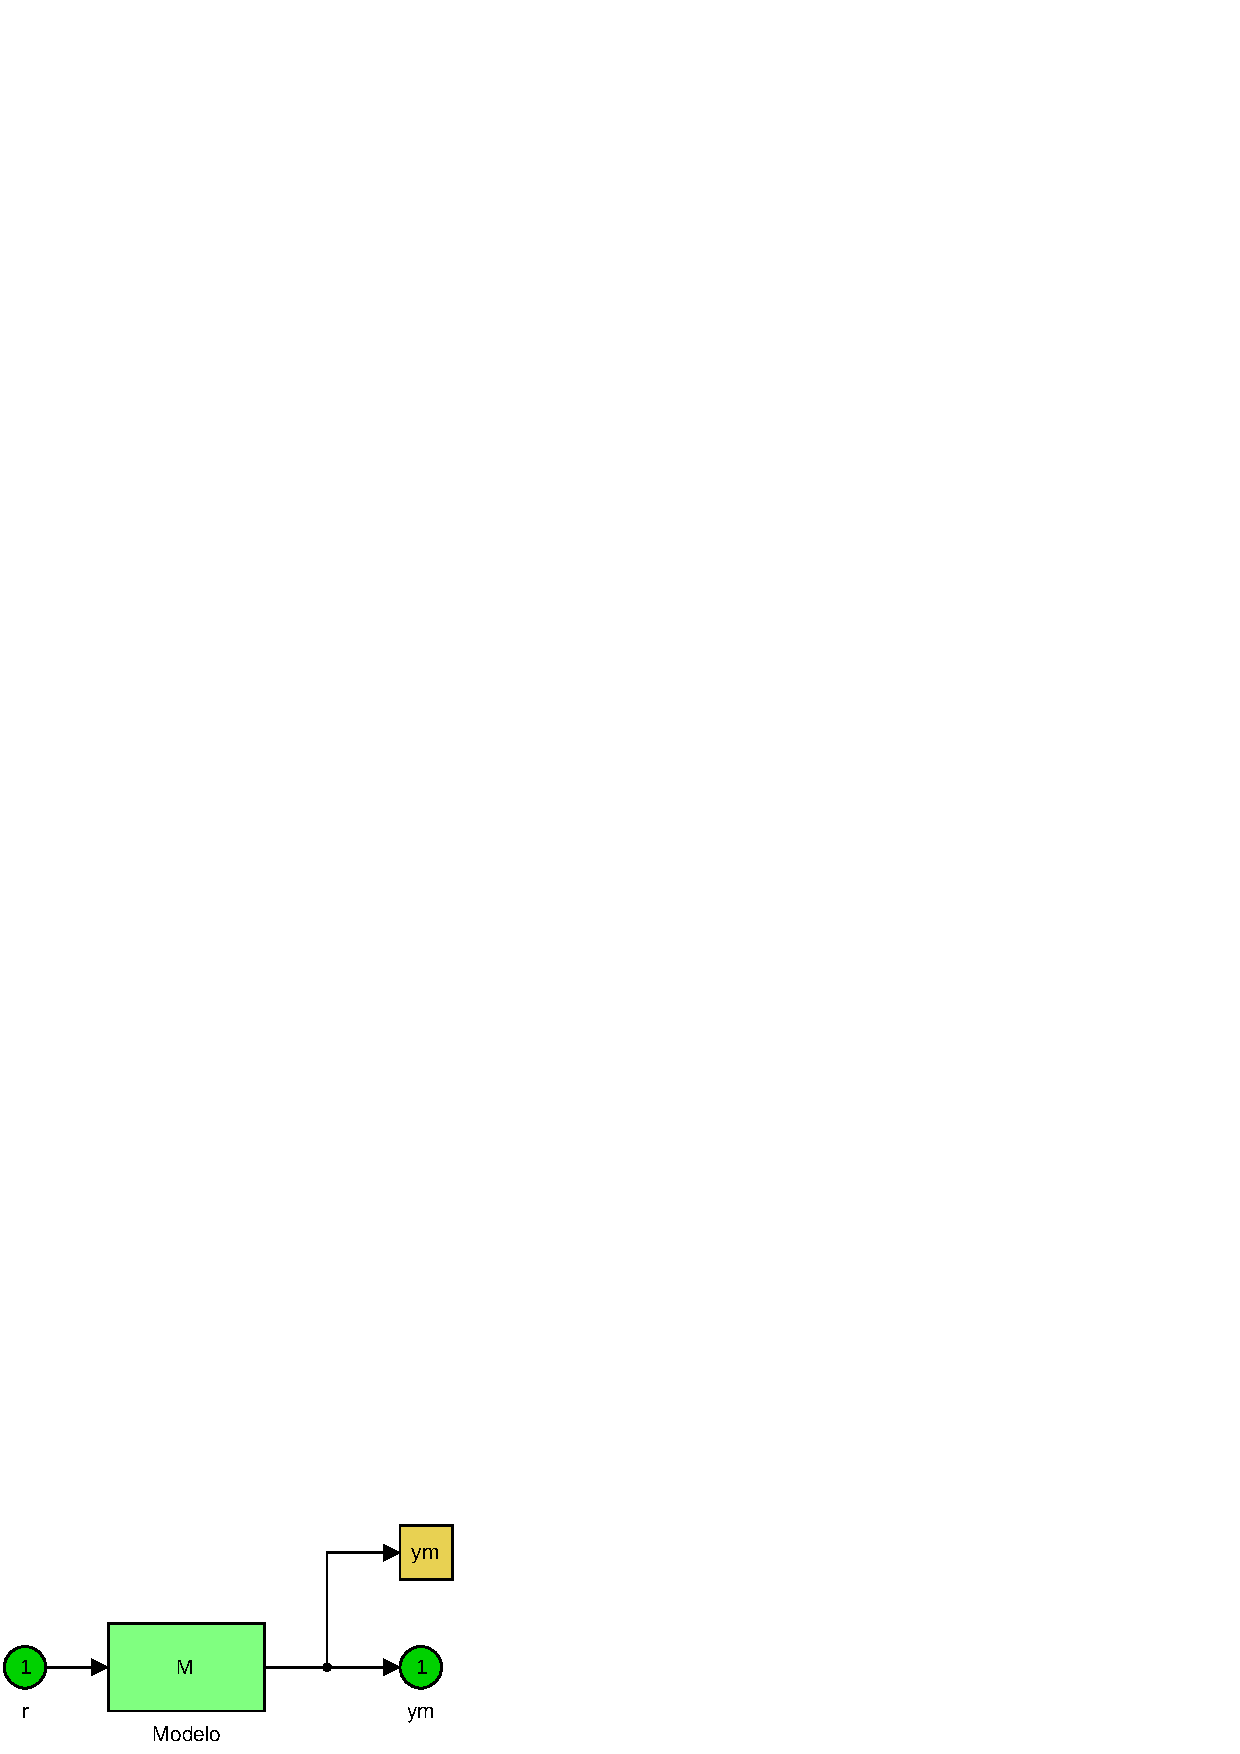
\includegraphics[scale=0.8]{figs/blocks/reference-model.pdf}
  \caption{Diagrama de blocos do modelo de refer�ncia.}
\end{figure}

%---------------------------------------------------------------------
\bigskip%
\begin{figure}[H]
  \centering
  \includegraphics[scale=0.8]{figs/blocks/reference-signal.pdf}
  \caption{Diagrama de blocos do gerador de sinais de refer�ncia.}
\end{figure}

%---------------------------------------------------------------------
\bigskip%
\begin{figure}[H]
  \centering
  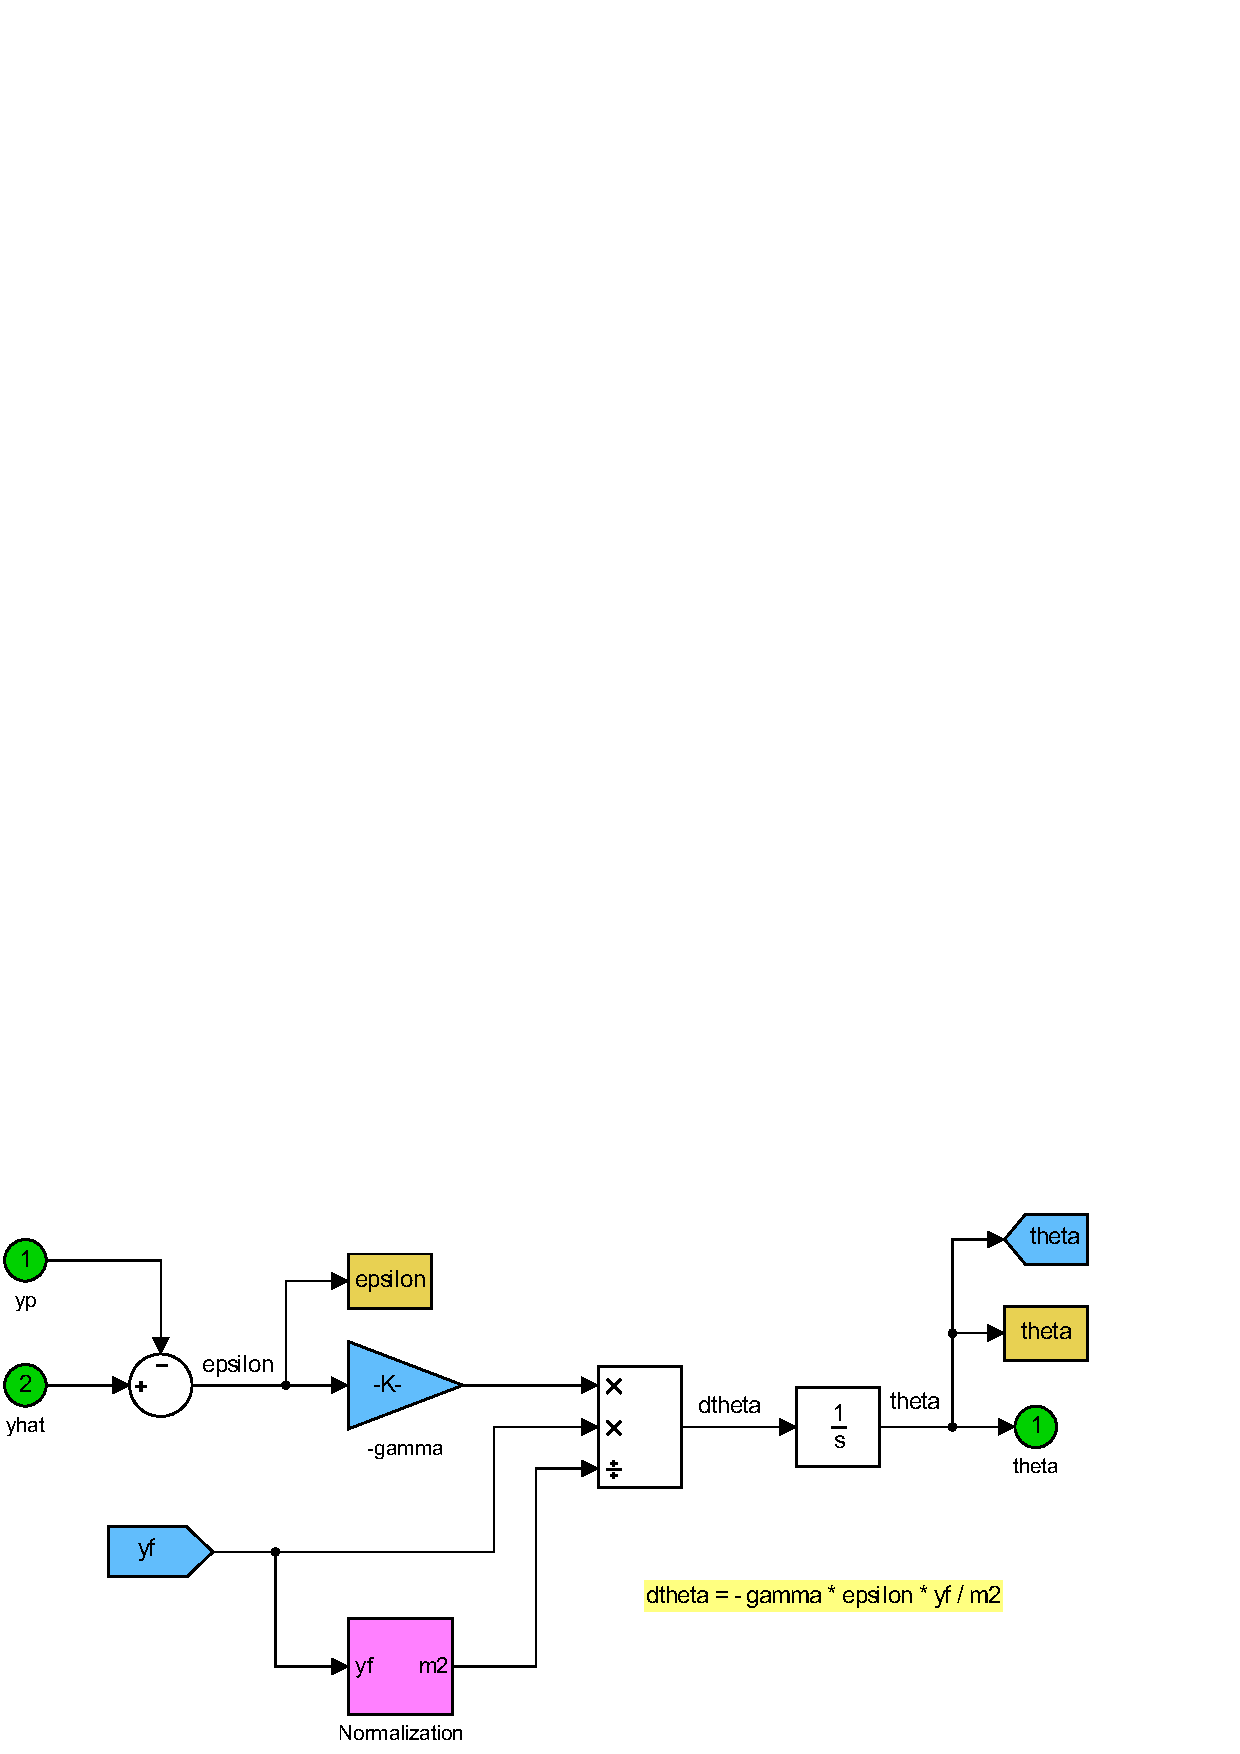
\includegraphics[width=16cm]{figs/blocks/adaptation.pdf}
  \caption{Diagrama de blocos da lei de adapta��o.}
\end{figure} \newpage
%---------------------------------------------------------------------
\section{Resultados das simula��es}

%Simula��o utilizando \HI{\texttt{Matlab/Simulink}}.

Nas simula��es, procuramos avaliar o comportamento do sistema para as seguintes condi��es:
%
\begin{enumerate*}[label=(\roman*)]
\item condi��o inicial $y(0)$;
\item p�lo (est�vel) do filtro $a_f$;
\item ganho de adapta��o $\gamma$.
\end{enumerate*}
%
Para cada simula��o, comparamos o comportamento das vari�veis do sistema para dois tipos de predi��o de sa�da $\hat{y}$:
%
\begin{enumerate*}[label=(\roman*)]
\item $\theta = \hat{a}_p + a_f$;
\item $\theta = \hat{a}_p$.
\end{enumerate*}

Apresentaremos os resultados obtidos atrav�s de simula��es no ambiente \HI{\texttt{Matlab/Simulink}} e os discutiremos na pr�xima se��o.

\subsection{Simula��o \#1}

Inicialmente, desejamos verificar o comportamento do sistema para varia��es no ganho de adapta��o $\gamma$.

%\bigskip%
%Par�metros e condi��es iniciais :
%
\begin{align*}
  a_p &= -2\,,  &  y_p(0) &= 0\,, & \theta(0) &= 0\,, \\
  a_m &= 1\,,   &  y_m(0) &= 0\,, & \gamma &= \HI{2, 100}\,, \\
  r &= 1\,, & a_f &= 1\,.
\end{align*}

\bigskip%
\begin{figure}[H]
  \centering
  \includegraphics[width=12cm]{figs/e0/gamma2gamma100.eps} \\[2mm]
\end{figure}

\begin{figure}[H]
  \centering
  \includegraphics[width=12cm]{figs/epsilon/gamma2gamma100.eps} 
\end{figure}


\begin{figure}[H]
  \centering
  \includegraphics[width=12cm]{figs/theta/gamma2gamma100.eps} 
\end{figure}

\begin{figure}[H]
  \centering
  \includegraphics[width=12cm]{figs/yp/gamma2gamma100.eps} 
\end{figure}

\begin{figure}[H]
  \centering
  \includegraphics[width=12cm]{figs/u/gamma2gamma100.eps} 
\end{figure}

\newpage%
%---------------------------------------------------------------------
\subsection{Simula��o \#2}

Na segunda simula��o, observamos o comportamento do sistema para varia��es no p�lo do filtro.

%\bigskip%
%Par�metros e condi��es iniciais:
%
\begin{align*}
  a_p &= -2\,,  &  y_p(0) &= 0\,, & \theta(0) &= 0\,, \\
  a_m &= 1\,,   &  y_m(0) &= 0\,, & \gamma &= 5\,, \\
  r &= 1\,, & a_f &= \HI{3, 5}\,.
\end{align*}

\begin{figure}[H]
  \centering
  \includegraphics[width=12cm]{figs/e0/af3af5.eps} \\[2mm]
\end{figure}

\begin{figure}[H]
  \centering
  \includegraphics[width=12cm]{figs/epsilon/af3af5.eps} 
\end{figure}


\begin{figure}[H]
  \centering
  \includegraphics[width=12cm]{figs/theta/af3af5.eps} 
\end{figure}

\begin{figure}[H]
  \centering
  \includegraphics[width=12cm]{figs/yp/af3af5.eps} 
\end{figure}

\begin{figure}[H]
  \centering
  \includegraphics[width=12cm]{figs/u/af3af5.eps} 
\end{figure}

\newpage%
%---------------------------------------------------------------------
\subsection{Simula��o \#3}

Na terceira simula��o, observamos o comportamento do sistema para varia��es no p�lo desconhecido da planta.

%\bigskip%
%Par�metros e condi��es iniciais:
%
\begin{align*}
  a_p &= \HI{-2, -5}\,,  &  y_p(0) &= 0\,, & \theta(0) &= 0\,, \\
  a_m &= 1\,,   &  y_m(0) &= 0\,, & \gamma &= 5\,, \\
  r &= 1\,, & a_f &= 1\,.
\end{align*}

\begin{figure}[H]
  \centering
  \includegraphics[width=12cm]{figs/e0/ap-2ap-5.eps} \\[2mm]
\end{figure}

\begin{figure}[H]
  \centering
  \includegraphics[width=12cm]{figs/epsilon/ap-2ap-5.eps} 
\end{figure}


\begin{figure}[H]
  \centering
  \includegraphics[width=12cm]{figs/theta/ap-2ap-5.eps} 
\end{figure}

\begin{figure}[H]
  \centering
  \includegraphics[width=12cm]{figs/yp/ap-2ap-5.eps} 
\end{figure}

\begin{figure}[H]
  \centering
  \includegraphics[width=12cm]{figs/u/ap-2ap-5.eps} 
\end{figure}

\newpage%
%---------------------------------------------------------------------

\subsection{Simula��o \#4}

Na simula��o 4, variamos o p�lo do modelo de refer�ncia utilizado.

%\bigskip%
%Par�metros e condi��es iniciais:
%
\begin{align*}
  a_p &= -2\,,  &  y_p(0) &= 0\,, & \theta(0) &= 0\,, \\
  a_m &= \HI{2, 5}\,,   &  y_m(0) &= 0\,, & \gamma &= 5\,, \\
  r &= 1\,, & a_f &= 1\,.
\end{align*}

\begin{figure}[H]
  \centering
  \includegraphics[width=12cm]{figs/e0/am2am5.eps} \\[2mm]
\end{figure}

\begin{figure}[H]
  \centering
  \includegraphics[width=12cm]{figs/epsilon/am2am5.eps} 
\end{figure}


\begin{figure}[H]
  \centering
  \includegraphics[width=12cm]{figs/theta/am2am5.eps} 
\end{figure}

\begin{figure}[H]
  \centering
  \includegraphics[width=12cm]{figs/yp/am2am5.eps} 
\end{figure}

\begin{figure}[H]
  \centering
  \includegraphics[width=12cm]{figs/u/am2am5.eps} 
\end{figure}

\newpage%
%---------------------------------------------------------------------

\subsection{Simula��o \#5}

Por �ltimo, observamos o comportamento do sistema para varia��es nas condi��es iniciais da planta.

%\bigskip%
%Par�metros e condi��es iniciais:
%
\begin{align*}
  a_p &= -2\,,  &  y_p(0) &= \HI{0, 5}\,, & \theta(0) &= 0\,, \\
  a_m &= 1\,,   &  y_m(0) &= 0\,, & \gamma &= 5\,, \\
  r &= 1\,, & a_f &= 1\,.
\end{align*}

\begin{figure}[H]
  \centering
  \includegraphics[width=12cm]{figs/e0/yp00yp05.eps} \\[2mm]
\end{figure}

\begin{figure}[H]
  \centering
  \includegraphics[width=12cm]{figs/epsilon/yp00yp05.eps} 
\end{figure}


\begin{figure}[H]
  \centering
  \includegraphics[width=12cm]{figs/theta/yp00yp05.eps} 
\end{figure}

\begin{figure}[H]
  \centering
  \includegraphics[width=12cm]{figs/yp/yp00yp05.eps} 
\end{figure}

\begin{figure}[H]
  \centering
  \includegraphics[width=12cm]{figs/u/yp00yp05.eps} 
\end{figure}

\newpage%
%---------------------------------------------------------------------
%---------------------------------------------------------------------
%\bibliographystyle{agsm}
%\bibliography{bib,coe736}

%---------------------------------------------------------------------
\end{document}
